\chapter{Optimal Transport and Wasserstein Distances}
\label{chap:optimal_transport}

\section{Introduction}
% Descriptive opening
Information theory provides a rich vocabulary for comparing probability distributions, primarily through divergences such as the Kullback-Leibler (KL) divergence and more generally, $f$-divergences (as explored in Chapter 23). However, these classical divergences suffer from a significant limitation when applied to the kinds of distributions often encountered in deep learning: they require distributions to have overlapping support. When comparing two distributions that are supported on disjoint, low-dimensional manifolds within a high-dimensional ambient space—a common scenario in generative modeling (the Manifold Hypothesis, Chapter 5)—the KL divergence is either undefined or infinite.

Consider the task of evaluating a generative model. We have a target distribution $P_{\text{data}}$ and a generated distribution $P_\theta$. If $P_{\text{data}}$ is a distribution over natural images, it resides on a thin manifold in the pixel space. Early in training, the generated distribution $P_\theta$ is likely supported on a completely different manifold. Because there is no intersection in their supports, the KL divergence provides no useful gradient signal to guide $P_\theta$ towards $P_{\text{data}}$. The divergence simply indicates that the distributions are completely different, without offering a metric of "how far apart" their respective manifolds lie in the ambient space.

This limitation motivates a shift from divergences based on point-wise density ratios to those based on the geometry of the underlying space. This brings us to the mathematical framework of \emph{Optimal Transport} (OT) and the resulting \emph{Wasserstein distances}. Intuitively, optimal transport frames the problem of comparing distributions as a logistics problem: if $P_\theta$ represents a pile of earth (or mass) and $P_{\text{data}}$ represents a hole of equal volume, what is the minimum cost required to transport the mass from $P_\theta$ to fill the hole at $P_{\text{data}}$? 

Because the cost of transport depends on the physical distance the mass must be moved in the ambient space (e.g., Euclidean distance), the Wasserstein distance naturally incorporates the geometry of the underlying metric space. It provides a smooth, meaningful measure of distance even between mutually singular distributions. In deep learning, this geometric awareness was famously leveraged to stabilize the training of Generative Adversarial Networks (GANs), leading to the Wasserstein GAN (WGAN). 

In this chapter, we rigorously develop the theory of optimal transport. We begin with the classical Monge formulation, transition to the Kantorovich relaxation, and define the Wasserstein distance. We then derive the Kantorovich-Rubinstein duality—the crucial mathematical result that makes the Wasserstein distance computationally tractable in deep learning via adversarial training.

\section{The Mathematical Core of Optimal Transport}

\subsection{The Monge Problem}
The study of optimal transport began with Gaspard Monge in 1781. Let $\mathcal{X}$ and $\mathcal{Y}$ be measurable spaces, which in the context of deep learning are typically subsets of $\mathbb{R}^d$. Let $P$ be a probability measure on $\mathcal{X}$ and $Q$ be a probability measure on $\mathcal{Y}$. We define a cost function $c: \mathcal{X} \times \mathcal{Y} \to \mathbb{R}_{\geq 0}$ representing the cost of moving a unit of mass from $x \in \mathcal{X}$ to $y \in \mathcal{Y}$.

A \emph{transport map} is a measurable function $T: \mathcal{X} \to \mathcal{Y}$. We say that $T$ pushes forward $P$ to $Q$, denoted as $T_{\#}P = Q$, if for every measurable set $A \subseteq \mathcal{Y}$, we have:
\[
P(T^{-1}(A)) = Q(A)
\]
The Monge problem seeks to find a transport map $T$ that minimizes the total cost of moving $P$ to $Q$:
\begin{definition}[Monge Problem]
\label{def:monge}
The Monge problem is to find a map $T^*$ such that
\[
T^* = \arg\inf_{T: T_{\#}P = Q} \int_{\mathcal{X}} c(x, T(x)) \, dP(x)
\]
\end{definition}

While intuitively appealing, the Monge problem suffers from severe structural flaws. Specifically, a transport map $T$ must be a deterministic function; it cannot split mass from a single point $x$ to multiple destinations in $\mathcal{Y}$. Consequently, if $P$ is a Dirac delta (a single point mass) and $Q$ is a mixture of two point masses, no valid map $T$ exists such that $T_{\#}P = Q$, rendering the feasible set empty.

\begin{figure}[h]
    \centering
    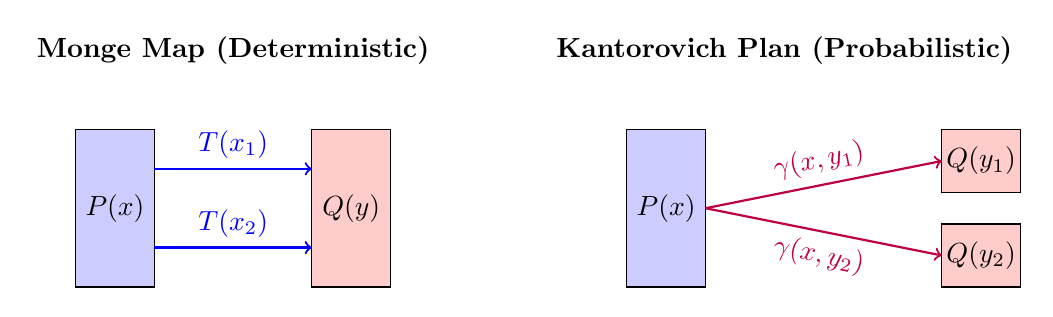
\begin{tikzpicture}
        % Monge Map
        \node at (0,3) {\textbf{Monge Map (Deterministic)}};
        \draw[fill=blue!20] (-2,0) rectangle (-1,2);
        \node at (-1.5,1) {$P(x)$};
        
        \draw[fill=red!20] (1,0) rectangle (2,2);
        \node at (1.5,1) {$Q(y)$};
        
        \draw[->, thick, blue] (-1, 1.5) -- (1, 1.5) node[midway, above] {$T(x_1)$};
        \draw[->, thick, blue] (-1, 0.5) -- (1, 0.5) node[midway, above] {$T(x_2)$};
        
        % Kantorovich Map
        \node at (7,3) {\textbf{Kantorovich Plan (Probabilistic)}};
        \draw[fill=blue!20] (5,0) rectangle (6,2);
        \node at (5.5,1) {$P(x)$};
        
        \draw[fill=red!20] (9,0) rectangle (10,0.8);
        \draw[fill=red!20] (9,1.2) rectangle (10,2);
        \node at (9.5,0.4) {$Q(y_2)$};
        \node at (9.5,1.6) {$Q(y_1)$};
        
        \draw[->, thick, purple] (6, 1) -- (9, 1.6) node[midway, above, sloped] {$\gamma(x, y_1)$};
        \draw[->, thick, purple] (6, 1) -- (9, 0.4) node[midway, below, sloped] {$\gamma(x, y_2)$};
    \end{tikzpicture}
    \caption{The Monge formulation requires deterministic mapping of mass, which can fail if mass must be split. The Kantorovich relaxation introduces a joint distribution (coupling) $\gamma$, allowing mass from a single source to be distributed across multiple targets.}
    \label{fig:monge_kantorovich}
\end{figure}

\subsection{The Kantorovich Relaxation}
To resolve the non-existence of solutions in the Monge problem, Leonid Kantorovich introduced a relaxation in 1942. Instead of finding a deterministic map $T$, Kantorovich proposed finding a \emph{coupling} or \emph{transport plan}—a joint probability measure $\gamma$ on $\mathcal{X} \times \mathcal{Y}$. 

Let $\Pi(P, Q)$ denote the set of all joint probability measures $\gamma$ on $\mathcal{X} \times \mathcal{Y}$ whose marginals are $P$ and $Q$. Mathematically, for any measurable sets $A \subseteq \mathcal{X}$ and $B \subseteq \mathcal{Y}$:
\[
\gamma(A \times \mathcal{Y}) = P(A) \quad \text{and} \quad \gamma(\mathcal{X} \times B) = Q(B)
\]

\begin{definition}[Kantorovich Problem]
\label{def:kantorovich}
The Kantorovich problem is to find a coupling $\gamma^* \in \Pi(P, Q)$ that minimizes the expected cost:
\[
\gamma^* = \arg\inf_{\gamma \in \Pi(P, Q)} \iint_{\mathcal{X} \times \mathcal{Y}} c(x, y) \, d\gamma(x, y)
\]
\end{definition}

The set $\Pi(P, Q)$ is never empty because the independent coupling $\gamma(x, y) = P(x)Q(y)$ always exists. Furthermore, because the objective function is linear in $\gamma$ and the constraint set $\Pi(P, Q)$ is convex and weakly compact, a minimum is guaranteed to exist under mild conditions (e.g., when cost $c$ is lower semi-continuous).

\subsection{The Wasserstein Distance}
When the spaces $\mathcal{X}$ and $\mathcal{Y}$ coincide and form a metric space $(\mathcal{X}, d)$, a natural choice for the cost function is the distance metric raised to a power $p \geq 1$: $c(x, y) = d(x, y)^p$. This choice leads to the formal definition of the Wasserstein distance.

\begin{definition}[$p$-Wasserstein Distance]
\label{def:wasserstein}
Let $(\mathcal{X}, d)$ be a Polish space (a separable completely metrizable space). For $p \geq 1$, the $p$-Wasserstein distance between two probability measures $P$ and $Q$ on $\mathcal{X}$ is defined as:
\[
W_p(P, Q) = \left( \inf_{\gamma \in \Pi(P, Q)} \iint_{\mathcal{X} \times \mathcal{X}} d(x, y)^p \, d\gamma(x, y) \right)^{1/p}
\]
\end{definition}

The Wasserstein distance $W_p$ is a true metric on the space of probability measures with finite $p$-th moments. 
In deep learning, the $1$-Wasserstein distance ($p=1$), often called the Earth Mover's Distance (EMD), is predominantly used. We will denote it simply as $W_1(P, Q)$.

\begin{theorem}[Weak Continuity of Wasserstein Distance]
Unlike the KL divergence, the Wasserstein distance metrizes weak convergence. A sequence of probability measures $(P_n)_{n \in \mathbb{N}}$ converges weakly to $P$ if and only if $W_p(P_n, P) \to 0$ (assuming uniformly integrable $p$-th moments).
\end{theorem}

\begin{proof}
The proof relies on the Portmanteau theorem and is standard in measure theory texts. The key implication for deep learning is that if a sequence of generated distributions $P_\theta$ smoothly approaches a target $P_{\text{data}}$, the Wasserstein distance smoothly decreases to zero, providing a continuous gradient $\nabla_\theta W_1(P_\theta, P_{\text{data}})$.
\end{proof}

\subsection{Numerical Example: Discrete Distributions}
Let us calculate $W_1$ for two simple discrete distributions on $\mathbb{R}$. 
Let $P = \frac{1}{2}\delta_0 + \frac{1}{2}\delta_2$ and $Q = \frac{1}{2}\delta_1 + \frac{1}{2}\delta_3$.
The cost metric is the Euclidean distance $d(x, y) = |x - y|$. 
The joint probability mass function (the coupling $\gamma$) can be represented as a $2 \times 2$ matrix, where rows correspond to the support of $P$ and columns to the support of $Q$. The marginals require row sums to be $1/2$ and column sums to be $1/2$.

The cost matrix $C$ where $C_{ij} = |x_i - y_j|$ is:
\[
C = \begin{pmatrix}
|0-1| & |0-3| \\
|2-1| & |2-3|
\end{pmatrix}
= \begin{pmatrix}
1 & 3 \\
1 & 1
\end{pmatrix}
\]
We want to minimize $\sum_{i,j} \gamma_{ij} C_{ij}$. Let the coupling matrix be $\Gamma$:
\[
\Gamma = \begin{pmatrix}
\gamma_{11} & \gamma_{12} \\
\gamma_{21} & \gamma_{22}
\end{pmatrix}
\]
To satisfy marginal constraints: $\gamma_{11} + \gamma_{12} = 1/2$, $\gamma_{21} + \gamma_{22} = 1/2$, $\gamma_{11} + \gamma_{21} = 1/2$, $\gamma_{12} + \gamma_{22} = 1/2$.
Notice that moving mass from $x=0$ to $y=1$ costs 1, and $x=2$ to $y=3$ costs 1. The total cost under the coupling $\Gamma = \begin{pmatrix} 1/2 & 0 \\ 0 & 1/2 \end{pmatrix}$ is:
\[
W_1(P, Q) = \frac{1}{2}(1) + 0(3) + 0(1) + \frac{1}{2}(1) = 1.
\]
Any other valid coupling, e.g., $\Gamma = \begin{pmatrix} 0 & 1/2 \\ 1/2 & 0 \end{pmatrix}$, yields a cost of $\frac{1}{2}(3) + \frac{1}{2}(1) = 2$. Thus, $W_1(P, Q) = 1$.

\subsection{Kantorovich-Rubinstein Duality}
Evaluating the primal Kantorovich problem directly in high dimensions is intractable due to the infinite-dimensional space of couplings $\Pi(P, Q)$. The pivotal breakthrough that allows Wasserstein distances to be used as objective functions in neural networks is the dual formulation.

\begin{theorem}[Kantorovich-Rubinstein Duality]
\label{thm:kr_duality}
For the $W_1$ distance, the Kantorovich problem admits the following dual representation:
\[
W_1(P, Q) = \sup_{\|f\|_L \leq 1} \mathbb{E}_{x \sim P}[f(x)] - \mathbb{E}_{y \sim Q}[f(y)]
\]
where the supremum is taken over all $1$-Lipschitz functions $f: \mathcal{X} \to \mathbb{R}$. A function $f$ is $1$-Lipschitz if $|f(x) - f(y)| \leq d(x, y)$ for all $x, y \in \mathcal{X}$.
\end{theorem}

\begin{proof}
Let us sketch the derivation using the min-max theorem. The primal problem is a constrained optimization problem. We can enforce the marginal constraints using Lagrange multipliers. Let $f \in L^1(dP)$ and $g \in L^1(dQ)$ be dual variables (functions). 
The Lagrangian is:
\begin{align*}
L(\gamma, f, g) &= \iint c(x,y) d\gamma(x,y) + \int f(x) \left( dP(x) - \int d\gamma(x,y) \right) + \int g(y) \left( dQ(y) - \int d\gamma(x,y) \right) \\
&= \int f(x) dP(x) + \int g(y) dQ(y) + \iint \left( c(x,y) - f(x) - g(y) \right) d\gamma(x,y)
\end{align*}
By the min-max theorem (Slater's condition holds), $\inf_\gamma \sup_{f,g} L = \sup_{f,g} \inf_\gamma L$.
When minimizing over $\gamma \geq 0$, if $c(x,y) - f(x) - g(y) < 0$ for any $x,y$, the inner infimum evaluates to $-\infty$. Therefore, we must constrain $f(x) + g(y) \leq c(x,y)$. Under this constraint, the integral with respect to $\gamma$ vanishes. The problem becomes:
\[
\sup_{f,g: f(x)+g(y) \leq c(x,y)} \int f(x) dP(x) + \int g(y) dQ(y)
\]
For $c(x,y) = d(x,y)$, one can show that the optimal $g$ is $-f$ ($c$-transform), and the constraint $f(x) - f(y) \leq d(x,y)$ implies exactly that $f$ is $1$-Lipschitz. This yields the Kantorovich-Rubinstein formula.
\end{proof}

This duality transforms the search over couplings into a maximization problem over a single scalar-valued function $f$, which in deep learning can be parameterized by a neural network.

\begin{figure}[h]
    \centering
    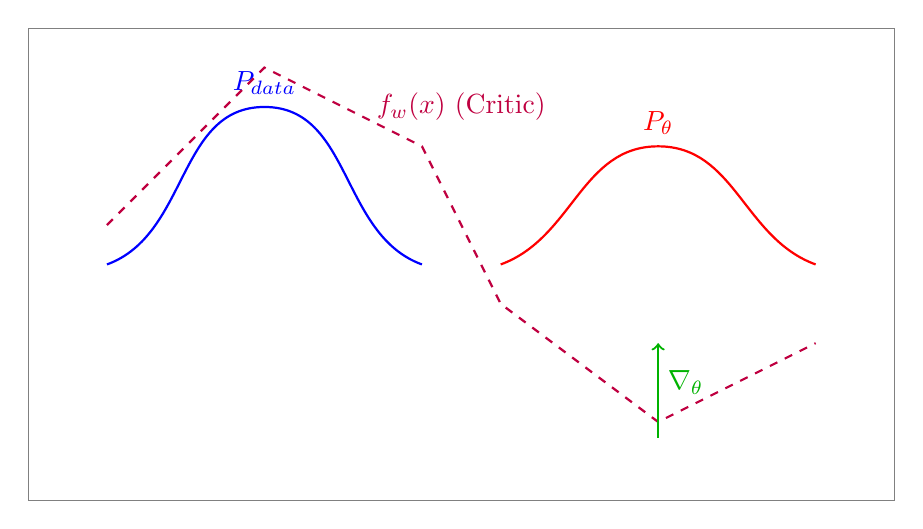
\begin{tikzpicture}
        % Distributions
        \draw[thick, blue] (0,0) to[out=20,in=180] (2,2) to[out=0,in=160] (4,0);
        \node[blue] at (2,2.3) {$P_{\text{data}}$};
        
        \draw[thick, red] (5,0) to[out=20,in=180] (7,1.5) to[out=0,in=160] (9,0);
        \node[red] at (7,1.8) {$P_\theta$};
        
        % Lipschitz function f
        \draw[thick, dashed, purple] (0, 0.5) -- (2, 2.5) -- (4, 1.5) -- (5, -0.5) -- (7, -2) -- (9, -1);
        \node[purple] at (4.5, 2) {$f_w(x)$ (Critic)};
        
        % Arrows indicating gradients
        \draw[->, thick, green!70!black] (7,-2.2) -- (7,-1);
        \node[green!70!black, right] at (7,-1.5) {$\nabla_\theta$};
        
        % Box
        \draw[gray, thin] (-1,-3) rectangle (10, 3);
    \end{tikzpicture}
    \caption{In the Wasserstein GAN framework, a neural network $f_w$ (the critic) acts as the dual function. It is trained to maximize the difference in expectations between $P_{\text{data}}$ and $P_\theta$ subject to a Lipschitz constraint. The gradients of this critic then smoothly push the generator's distribution $P_\theta$ towards $P_{\text{data}}$.}
    \label{fig:wgan_critic}
\end{figure}

In the context of the Wasserstein GAN, the function $f$ (often parameterized with weights $w$, so $f_w$) is called the \emph{critic} rather than the discriminator, because it outputs a real-valued score rather than a probability. The generator, parametrized by $\theta$, minimizes the Wasserstein distance estimated by the critic.

\section{Horizon}
\begin{horizon}
The mathematical elegance of the Kantorovich-Rubinstein duality fundamentally reoriented generative modeling. However, enforcing the $1$-Lipschitz constraint globally on a neural network remains a severe theoretical and practical challenge. Existing methods, such as gradient penalty or weight normalization, enforce the constraint only locally along the interpolation path or restrict the capacity of the network in poorly understood ways.

It is conjectured that the set of functions achievable by standard deep neural networks (with ReLU or similar piecewise linear activations) under strict global Lipschitz bounds may be pathologically constrained, lacking the expressivity to accurately compute the supremum in the dual formulation for complex distributions. An open question is whether a fundamentally different architecture or parameterization could perfectly capture the space of $1$-Lipschitz functions in high dimensions without collapsing the model's capacity.

Future work might show that alternative geometric formulations, such as those relying on entropic regularization (e.g., the Sinkhorn divergence), will supersede the strict dual approach. Entropic OT replaces the hard Lipschitz constraint with a soft entropic penalty, yielding computationally robust, differentiable distance metrics that naturally interpolate between maximum mean discrepancy and optimal transport, potentially providing the definitive metric space for the next generation of deep learning representations.
\end{horizon}

\section{Summary and Exercises}
In this chapter, we identified the failure modes of density-based divergences when dealing with mutually singular distributions supported on disjoint manifolds. We formalized the geometry-aware framework of optimal transport, beginning with the restrictive Monge problem and moving to the probabilistically relaxed Kantorovich formulation. By defining the Wasserstein distance and leveraging the Kantorovich-Rubinstein duality, we established a tractable objective function that computes continuous gradients even when distributions do not overlap.

\subsection*{Exercises}
\begin{enumerate}
    \item \textbf{Translation Invariance:} Prove that for a shift $c \in \mathbb{R}^d$, $W_p(P, Q) = W_p(P_c, Q_c)$ where $P_c$ is the distribution of $X+c$ for $X \sim P$.
    \item \textbf{The 1D Case:} For continuous distributions on the real line $\mathbb{R}$ with cumulative distribution functions $F(x)$ and $G(y)$, prove that the $p$-Wasserstein distance has the closed-form solution:
    \[ W_p^p(P, Q) = \int_0^1 |F^{-1}(u) - G^{-1}(u)|^p \, du \]
    where $F^{-1}$ and $G^{-1}$ are the quantile functions.
    \item \textbf{Lipschitz Enforcement:} Compare clipping weights (as originally proposed in WGAN) versus gradient penalty ($L= (\|\nabla f(x)\|_2 - 1)^2$) in terms of bounding the Lipschitz constant of $f$. Why does weight clipping artificially constrain the functional capacity more severely?
\end{enumerate}

% TODO-CITE: Ensure all named results are cited.
